\documentclass[journal,12pt,twocolumn]{IEEEtran}
%
\usepackage{setspace}
%eghskljfnd
\usepackage{gensymb}
\usepackage{xcolor}
\usepackage{caption}
%\usepackage{subcaption}
%\doublespacing
\singlespacing

%\usepackage{graphicx}
%\usepackage{amssymb}
%\usepackage{relsize}
\usepackage[cmex10]{amsmath}
\usepackage{mathtools}
%\usepackage{amsthm}
%\interdisplaylinepenalty=2500
%\savesymbol{iint}
%\usepackage{txfonts}
%\restoresymbol{TXF}{iint}
%\usepackage{wasysym}
\usepackage{hyperref}
\usepackage{amsthm}
\usepackage{mathrsfs}
\usepackage{txfonts}
\usepackage{stfloats}
\usepackage{cite}
\usepackage{cases}
\usepackage{subfig}
%\usepackage{xtab}
\usepackage{longtable}
\usepackage{multirow}
%\usepackage{algorithm}
%\usepackage{algpseudocode}
%\usepackage{enumerate}
\usepackage{enumitem}
\usepackage{mathtools}
%\usepackage{iithtlc}
%\usepackage[framemethod=tikz]{mdframed}
\usepackage{listings}


%\usepackage{stmaryrd}

\usepackage{draftwatermark}
\SetWatermarkLightness{ 0.85 }
\SetWatermarkText{EE3900}
\SetWatermarkScale{1}
%\usepackage{wasysym}
%\newcounter{MYtempeqncnt}
\DeclareMathOperator*{\Res}{Res}
%\renewcommand{\baselinestretch}{2}
\renewcommand\thesection{\arabic{section}}
\renewcommand\thesubsection{\thesection.\arabic{subsection}}
\renewcommand\thesubsubsection{\thesubsection.\arabic{subsubsection}}

\renewcommand\thesectiondis{\arabic{section}}
\renewcommand\thesubsectiondis{\thesectiondis.\arabic{subsection}}
\renewcommand\thesubsubsectiondis{\thesubsectiondis.\arabic{subsubsection}}

%\renewcommand{\labelenumi}{\textbf{\theenumi}}
%\renewcommand{\theenumi}{P.\arabic{enumi}}

% correct bad hyphenation here
\hyphenation{op-tical net-works semi-conduc-tor}

\lstset{
language=Python,
frame=single, 
breaklines=true,
columns=fullflexible
}



\begin{document}
%

\theoremstyle{definition}
\newtheorem{theorem}{Theorem}[section]
\newtheorem{problem}{Problem}
\newtheorem{proposition}{Proposition}[section]
\newtheorem{lemma}{Lemma}[section]
\newtheorem{corollary}[theorem]{Corollary}
\newtheorem{example}{Example}[section]
\newtheorem{definition}{Definition}[section]
%\newtheorem{algorithm}{Algorithm}[section]
%\newtheorem{cor}{Corollary}
\newcommand{\BEQA}{\begin{eqnarray}}
          \newcommand{\EEQA}{\end{eqnarray}}
\newcommand{\define}{\stackrel{\triangle}{=}}

\bibliographystyle{IEEEtran}
%\bibliographystyle{ieeetr}

\providecommand{\nCr}[2]{\,^{#1}C_{#2}} % nCr
\providecommand{\nPr}[2]{\,^{#1}P_{#2}} % nPr
\providecommand{\mbf}{\mathbf}
\providecommand{\pr}[1]{\ensuremath{\Pr\left(#1\right)}}
\providecommand{\qfunc}[1]{\ensuremath{Q\left(#1\right)}}
\providecommand{\sbrak}[1]{\ensuremath{{}\left[#1\right]}}
\providecommand{\lsbrak}[1]{\ensuremath{{}\left[#1\right.}}
\providecommand{\rsbrak}[1]{\ensuremath{{}\left.#1\right]}}
\providecommand{\brak}[1]{\ensuremath{\left(#1\right)}}
\providecommand{\lbrak}[1]{\ensuremath{\left(#1\right.}}
\providecommand{\rbrak}[1]{\ensuremath{\left.#1\right)}}
\providecommand{\cbrak}[1]{\ensuremath{\left\{#1\right\}}}
\providecommand{\lcbrak}[1]{\ensuremath{\left\{#1\right.}}
\providecommand{\rcbrak}[1]{\ensuremath{\left.#1\right\}}}
\theoremstyle{remark}
\newtheorem{rem}{Remark}
\newcommand{\sgn}{\mathop{\mathrm{sgn}}}
\providecommand{\abs}[1]{\left\vert#1\right\vert}
\providecommand{\res}[1]{\Res\displaylimits_{#1}}
\providecommand{\norm}[1]{\lVert#1\rVert}
\providecommand{\mtx}[1]{\mathbf{#1}}
\providecommand{\mean}[1]{E\left[ #1 \right]}
\providecommand{\fourier}{\overset{\mathcal{F}}{ \rightleftharpoons}}
\providecommand{\ztrans}{\overset{\mathcal{Z}}{ \rightleftharpoons}}

%\providecommand{\hilbert}{\overset{\mathcal{H}}{ \rightleftharpoons}}
\providecommand{\system}{\overset{\mathcal{H}}{ \longleftrightarrow}}
%\newcommand{\solution}[2]{\textbf{Solution:}{#1}}
\newcommand{\solution}{\noindent \textbf{Solution: }}
\providecommand{\dec}[2]{\ensuremath{\overset{#1}{\underset{#2}{\gtrless}}}}
\numberwithin{equation}{section}
%\numberwithin{equation}{subsection}
%\numberwithin{problem}{subsection}
%\numberwithin{definition}{subsection}
\makeatletter
\@addtoreset{figure}{problem}
\makeatother

\let\StandardTheFigure\thefigure
%\renewcommand{\thefigure}{\theproblem.\arabic{figure}}
\renewcommand{\thefigure}{\theproblem}


%\numberwithin{figure}{subsection}

\def\putbox#1#2#3{\makebox[0in][l]{\makebox[#1][l]{}\raisebox{\baselineskip}[0in][0in]{\raisebox{#2}[0in][0in]{#3}}}}
\def\rightbox#1{\makebox[0in][r]{#1}}
\def\centbox#1{\makebox[0in]{#1}}
\def\topbox#1{\raisebox{-\baselineskip}[0in][0in]{#1}}
\def\midbox#1{\raisebox{-0.5\baselineskip}[0in][0in]{#1}}

\vspace{3cm}

\title{
     %\logo{
     Digital Signal Processing
     %}
     %	\logo{Octave for Math Computing }
}
%\title{
%	\logo{Matrix Analysis through Octave}{\begin{center}\includegraphics[scale=.24]{tlc}\end{center}}{}{HAMDSP}
%}


% paper title
% can use linebreaks \\ within to get better formatting as desired
%\title{Matrix Analysis through Octave}
%
%
% author names and IEEE memberships
% note positions of commas and nonbreaking spaces ( ~ ) LaTeX will not break
% a structure at a ~ so this keeps an author's name from being broken across
% two lines.
% use \thanks{} to gain access to the first footnote area
% a separate \thanks must be used for each paragraph as LaTeX2e's \thanks
% was not built to handle multiple paragraphs
%

\author{ Shivanshu \\ AI21bBTECH11027 %<-this  stops a space
     \thanks{*The author is a student with the Department
          of Artificial Intelligence, Indian Institute of Technology, Hyderabad
          502285 India e-mail:  ai21btech11027@iith.ac.in
          .}% <-this % stops a space
     %\thanks{J. Doe and J. Doe are with Anonymous University.}% <-this % stops a space
     %\thanks{Manuscript received April 19, 2005; revised January 11, 2007.}}
}
% note the % following the last \IEEEmembership and also \thanks - 
% these prevent an unwanted space from occurring between the last author name
% and the end of the author line. i.e., if you had this:
% 
% \author{....lastname \thanks{...} \thanks{...} }
%                     ^------------^------------^----Do not want these spaces!
%
% a space would be appended to the last name and could cause every name on that
% line to be shifted left slightly. This is one of those "LaTeX things". For
% instance, "\textbf{A} \textbf{B}" will typeset as "A B" not "AB". To get
% "AB" then you have to do: "\textbf{A}\textbf{B}"
% \thanks is no different in this regard, so shield the last } of each \thanks
% that ends a line with a % and do not let a space in before the next \thanks.
% Spaces after \IEEEmembership other than the last one are OK (and needed) as
% you are supposed to have spaces between the names. For what it is worth,
% this is a minor point as most people would not even notice if the said evil
% space somehow managed to creep in.



% The paper headers
%\markboth{Journal of \LaTeX\ Class Files,~Vol.~6, No.~1, January~2007}%
%{Shell \MakeLowercase{\textit{et al.}}: Bare Demo of IEEEtran.cls for Journals}
% The only time the second header will appear is for the odd numbered pages
% after the title page when using the twoside option.
% 
% *** Note that you probably will NOT want to include the author's ***
% *** name in the headers of peer review papers.                   ***
% You can use \ifCLASSOPTIONpeerreview for conditional compilation here if
% you desire.




% If you want to put a publisher's ID mark on the page you can do it like
% this:
%\IEEEpubid{0000--0000/00\$00.00~\copyright~2007 IEEE}
% Remember, if you use this you must call \IEEEpubidadjcol in the second
% column for its text to clear the IEEEpubid mark.

\pagecolor{cyan!20!white}
\newcommand{\myvec}[1]{\ensuremath{\begin{pmatrix}#1\end{pmatrix}}}
% make the title area
\maketitle

%\newpage

\tableofcontents

%\renewcommand{\thefigure}{\thesection.\theenumi}
%\renewcommand{\thetable}{\thesection.\theenumi}

\renewcommand{\thefigure}{\theenumi}
\renewcommand{\thetable}{\theenumi}

%\renewcommand{\theequation}{\thesection}


\bigskip

\begin{abstract}
     This manual provides a simple introduction to digital signal processing.
\end{abstract}
\section{Software Installation}
Run the following commands
\begin{lstlisting}
sudo apt-get update
sudo apt-get install libffi-dev libsndfile1 python3-scipy  python3-numpy python3-matplotlib 
sudo pip install cffi pysoundfile 
\end{lstlisting}
\section{Digital Filter}
\begin{enumerate}[label=\thesection.\arabic*
          ,ref=\thesection.\theenumi]
     \item
           \label{prob:input}
           Download the sound file from
           \begin{lstlisting}
wget https://github.com/Shivanshu8211/EE3900/blob/master/codes/Sound_Noise.wav
\end{lstlisting}
           %\href{http://tlc.iith.ac.in/img/sound/Sound_Noise.wav}{\url{http://tlc.iith.ac.in/img/sound/Sound_Noise.wav}}  
           %in the link given below.
           %\linebreak
     \item
           \label{prob:spectrogram}
           You will find a spectrogram at \href{https://academo.org/demos/spectrum-analyzer}{\url{https://academo.org/demos/spectrum-analyzer}}.
           %\end{problem}
           %%
           %
           %%\onecolumn
           %%\input{./figs/fir}
           %\begin{problem}
           Upload the sound file that you downloaded in Problem \ref{prob:input} in the spectrogram  and play.  Observe the spectrogram. What do you find?
           \\
           %
           \solution There are a lot of yellow lines between 440 Hz to 5.1 KHz.  These represent the synthesizer key tones. Also, the key strokes
           are audible along with background noise.
           % By observing spectrogram, it clearly shows that tonal frequency is under 4kHz. And above 4kHz only noise is present.
     \item
           \label{prob:output}
           Write the python code for removal of out of band noise and execute the code.
           \\
           \solution
           \lstinputlisting{./codes/Cancel_noise.py}
           %\begin{figure}[h]
           %\centering
           %\includegraphics[width=\columnwidth]{enc_block_diag.png}
           %\caption{}
           %\label{fig:convolution encoder}
           %\end{figure}
           %\input{block_enc}
     \item
           The output of the python script in Problem \ref{prob:output} is the audio file Sound\_With\_ReducedNoise.wav. Play the file in the spectrogram in Problem \ref{prob:spectrogram}. What do you observe?
           \\
           \solution The key strokes as well as background noise is subdued in the audio.  Also,  the signal is blank for frequencies above 5.1 kHz.

\end{enumerate}
\section{Difference Equation}
\begin{enumerate}[label=\thesection.\arabic*,ref=\thesection.\theenumi]
     \item Let
           \begin{equation}
                x(n) = \cbrak{\underset{\uparrow}{1},2,3,4,2,1}
           \end{equation}
           Sketch $x(n)$. \\
           \solution Graph of x(n) has been plotted in part 1 of Fig. \ref{fig:xnyn}.
     \item Let
           \begin{multline}
                \label{eq:iir_filter}
                y(n) + \frac{1}{2}y(n-1) = x(n) + x(n-2),
                \\
                y(n) = 0, n < 0
           \end{multline}
           Sketch $y(n)$.
           \\
           \solution The following code yields Fig. \ref{fig:xnyn}.
           \begin{lstlisting}
wget https://github.com/Shivanshu8211/EE3900/blob/master/codes/xnyn.py
\end{lstlisting}
           \begin{figure}[!ht]
                \begin{center}
                     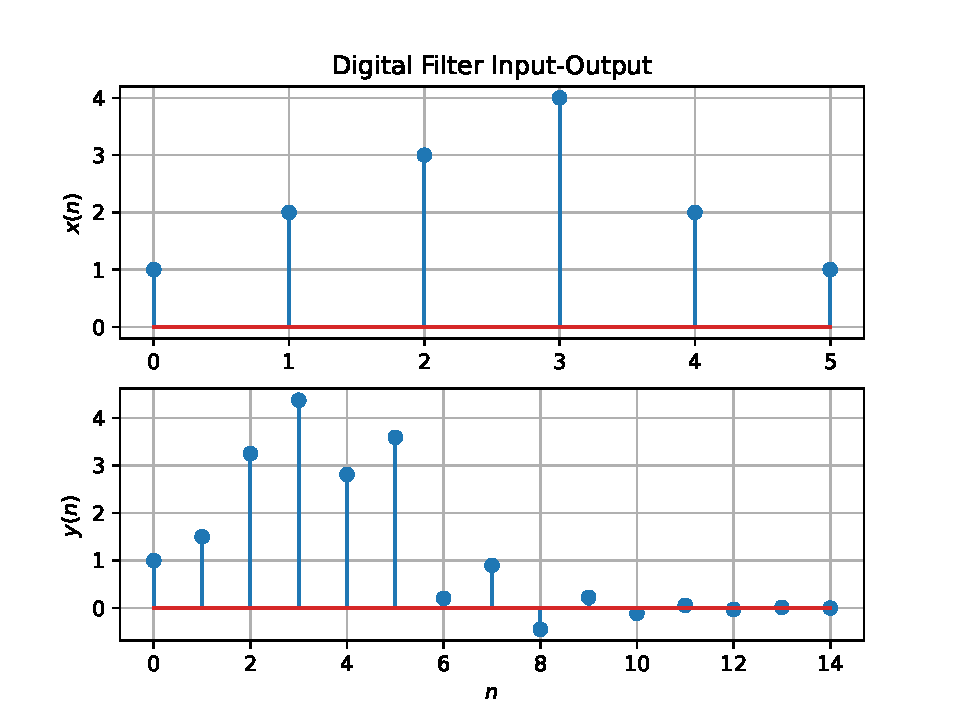
\includegraphics[width=\columnwidth]{./figs/xnyn}
                \end{center}
                \captionof{figure}{}
                \label{fig:xnyn}
           \end{figure}
     \item Repeat the above exercise using a C code.
           \solution The following code is in c and doing the same function as the above one is doing.
           \begin{lstlisting}
wget https://github.com/Shivanshu8211/EE3900/blob/master/codes/xnyn.c
           \end{lstlisting}
\end{enumerate}
\section{$Z$-transform}
\begin{enumerate}[label=\thesection.\arabic*]
     \item The $Z$-transform of $x(n)$ is defined as
           %
           \begin{equation}
                \label{eq:z_trans}
                X(z)={\mathcal {Z}}\{x(n)\}=\sum _{n=-\infty }^{\infty }x(n)z^{-n}
           \end{equation}
           %
           Show that
           \begin{equation}
                \label{eq:shift1}
                {\mathcal {Z}}\{x(n-1)\} = z^{-1}X(z)
           \end{equation}
           and find
           \begin{equation}
                {\mathcal {Z}}\{x(n-k)\}
           \end{equation}
           \solution Given that,
           \begin{align}
                X\brak{z} & = \mathcal{Z}\cbrak{x\brak{n}}               \\
                          & = \sum_{n = -\infty}^{\infty}x\brak{n}z^{-n}
           \end{align}
           So,
           \begin{align}
                \mathcal{Z}\cbrak{x\brak{n-1}} & = \sum_{n=-\infty}^{\infty}x\brak{n-1}z^{-n}
           \end{align}
           let $n-1 = k$,
           \begin{align}
                 & = \sum_{k=-\infty}^{\infty}x\brak{k}z^{-\brak{k+1}} \\
                 & = z^{-1}\sum_{k=-\infty}^{\infty}x\brak{k}z^{-k}    \\
                 & = z^{-1}\sum_{n=-\infty}^{\infty}x\brak{n}z^{-n}    \\
                 & = z^{-1}X\brak{z}
           \end{align}
           From \eqref{eq:z_trans},
           \begin{align}
                {\mathcal {Z}}\{x(n-k)\} & =\sum _{n=-\infty }^{\infty }x(n-1)z^{-n}
                \\
                                         & =\sum _{n=-\infty }^{\infty }x(n)z^{-n-1} = z^{-1}\sum _{n=-\infty }^{\infty }x(n)z^{-n}
           \end{align}
           \begin{equation}
                \label{eq:z_trans_shift}
                {\mathcal {Z}}\{x(n-k)\} = z^{-k}X(z)
           \end{equation}
           Hence proved.
     \item Obtain X(z) for x(n) defined in problem 3.1.
           \solution Given
           \begin{equation}
                x(n) = \cbrak{\underset{\uparrow}{1},2,3,4,2,1}
           \end{equation}
           and the $Z$-transform of $x(n)$ is defined as
           \begin{align}
                X(z)                       & = \sum _{n=-\infty }^{\infty }x(n)z^{-n}                 \\
                \sum _{n=0 }^{5}x(n)z^{-n} & = z^{0} + 2z^{-1} + 3z^{-2} + 4z^{-3} + 2z^{-4} + z^{-5}
           \end{align}

     \item Find
           %
           \begin{equation}
                \label{eq:dtft_1}
                H(z) = \frac{Y(z)}{X(z)}
           \end{equation}
           %
           from  $\eqref{eq:iir_filter}$ assuming that the $Z$-transform is a linear operation.
           \\
           \solution since $Z$-transform is a linear operator therefore \\
           y(z) = Y(z) and x(z) = X(z) \\
           So, \\
           on applying \eqref{eq:z_trans_shift} in \eqref{eq:iir_filter},
           we get
           \begin{align}
                Y(z) + \frac{1}{2}z^{-1}Y(z) & = X(z)+z^{-2}X(z)
                \\
                \implies \frac{Y(z)}{X(z)}   & = \frac{1 + z^{-2}}{1 + \frac{1}{2}z^{-1}}
                \label{eq:freq_resp}
           \end{align}

     \item Find the Z transform of
           \begin{equation}
                \delta(n)
                =
                \begin{cases}
                     1 & n = 0
                     \\
                     0 & \text{otherwise}
                \end{cases}
           \end{equation}
           and show that the $Z$-transform of
           \begin{equation}
                \label{eq:unit_step}
                u(n)
                =
                \begin{cases}
                     1 & n \ge 0
                     \\
                     0 & \text{otherwise}
                \end{cases}
           \end{equation}
           is
           \begin{equation}
                U(z) = \frac{1}{1-z^{-1}}, \quad \abs{z} > 1
           \end{equation}
           \solution
           The $Z$-transform of $\delta{n}$ is,
           \begin{align}
                \mathcal{Z}\cbrak{\delta{n}} & = \sum_{n=-\infty}^{\infty}\delta\brak{n}z^{-n} \\
                                             & = \delta\brak{0}z^{0}                           \\
                                             & = 1
           \end{align}
           and the $Z$-transform of unit-step function $u\brak{n}$ is,
           \begin{align}
                U\brak{n} & = \sum_{n=-\infty}^{\infty}u\brak{n}z^{-n} \\
                          & = 0 + \sum_{n = 0}^{\infty}1.z^{-n}        \\
                          & = 1 + z^{-1} + z^{-2} + .\,.\,.
           \end{align}
           and from \eqref{eq:unit_step},
           \begin{align}
                U(z) & = \sum _{n= 0}^{\infty}z^{-n}
                \\
                     & =\frac{1}{1-z^{-1}}, \quad \abs{z} > 1
           \end{align}
           using the fomula for the sum of an infinite geometric progression.
           %
     \item Show that
           \begin{equation}
                \label{eq:anun}
                a^nu(n) \ztrans \frac{1}{1-az^{-1}} \quad \abs{z} > \abs{a}
           \end{equation}
           \solution
           The $Z$- transform will be
           \begin{align}
                \mathcal{Z}\cbrak{a^nu\brak{n}} & = \sum_{n = 0}^{\infty}a^{n}z^{-n}                    \\
                                                & = 1 + \frac{a}{z} + \brak{\frac{a}{z}}^2 + .\,.\,.\,.
           \end{align}
           Above is a infinite geometric series with first term $1$ and common ratio as $\frac{a}{z}$ and it can
           be written as,
           \begin{align}
                \mathcal{Z}\cbrak{a^nu\brak{n}} & = \frac{1}{1 - \frac{a}{z}} \because \abs{a} < \abs{z}
           \end{align}
           Therefore,
           \begin{equation}
                a^nu(n) \ztrans \frac{1}{1-az^{-1}} \quad \abs{z} > \abs{a}
           \end{equation}
           %
     \item
           Let
           \begin{equation}
                H\brak{e^{j \omega}} = H\brak{z = e^{j \omega}}.
           \end{equation}
           Plot $\abs{H\brak{e^{j \omega}}}$.  Comment.  $H(e^{j \omega})$ is known as the {\em Discret Time Fourier Transform} (DTFT) of $h(n)$.\\
           \solution
           Download the code for the plot $\ref{DTFT}$ from the link below
           \begin{lstlisting}
               wget https://github.com/Shivanshu8211/EE3900/blob/master/codes/dtft.py
               \end{lstlisting}
           \begin{figure}[!ht]
                \centering
                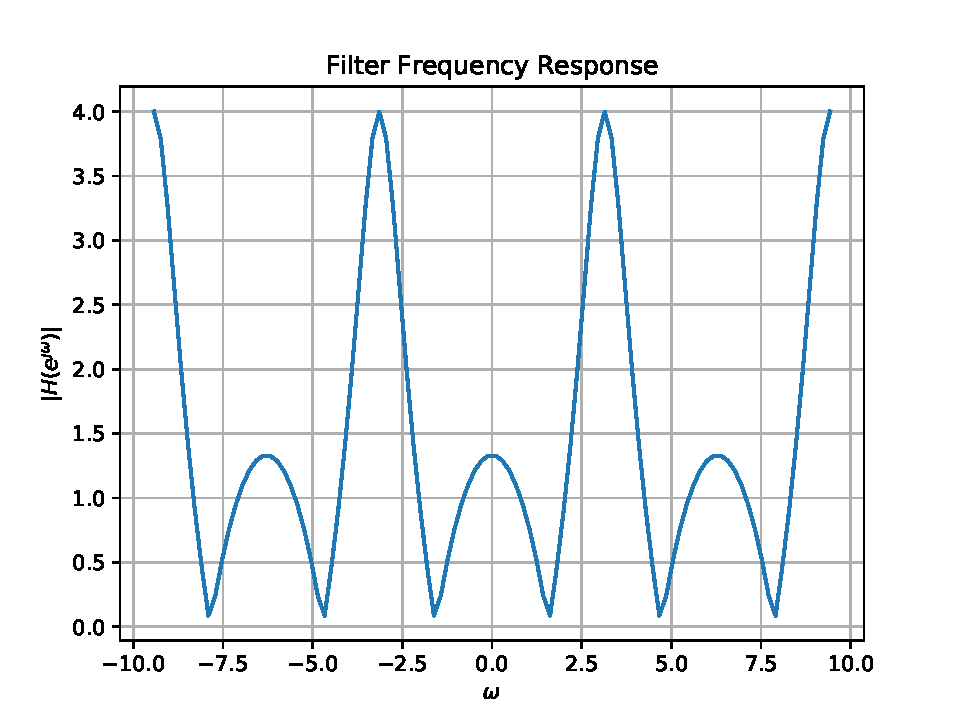
\includegraphics[width=\columnwidth]{./figs/dtft}
                \caption{$\abs{H\brak{e^{\j\omega}}}$}
                \label{fig:dtft}
           \end{figure}
           Now using $\eqref{eq:freq_resp}$, we will find $\abs{H\brak{e^{j \omega}}}$,
           \begin{align}
                H\brak{e^{j \omega}}                  & = \frac{1+e^{-2j\omega}}{1 + \frac{e^{-j\omega}}{2}}                                                                              \\
                \implies \abs{H\brak{e^{j \omega}}}   & = \frac{\abs{1+e^{-2j\omega}}}{\abs{1 + \frac{e^{-j\omega}}{2}}}                                                                  \\
                                                      & = \frac{\abs{1+e^{2j\omega}}}{\abs{e^{2j\omega} + \frac{e^{j\omega}}{2}}}                                                         \\
                                                      & = \frac{\abs{1+\cos2\omega + j\sin2\omega}}{\abs{e^{j\omega}+ \frac{1}{2}}}                                                       \\
                                                      & = \frac{\abs{4\cos^2\brak{\omega} + 4j\sin\brak{\omega}\cos\brak{\omega}}}{\abs{2e^{j\omega} + 1}}                                \\
                                                      & = \frac{\abs{4\cos\brak{\omega}}\abs{\cos\brak{\omega} + j\sin\brak{\omega}}}{\abs{2\cos\brak{\omega} + 1 + 2j\sin\brak{\omega}}} \\
                \therefore \abs{H\brak{e^{j \omega}}} & = \frac{\abs{4\cos\brak{\omega}}}{\sqrt{5 +4\cos\brak{\omega}}}
           \end{align}
           Since $\abs{H(e^{j\omega})}$ is function of cosine we can say it is periodic.And from the plot $\ref{DTFT}$ we can say that it is symmetric about $\omega = 0\brak{\text{even function}}$ and it is periodic with period $2\pi$.You can find the same from the theoritical expression $\abs{H\brak{e^{j \omega}}}$,
           \begin{align}
                H(e^{j\omega}) & = H(e^{j(-\omega)})\brak{\text{cos is an even function}}
           \end{align}
           And to find period, the period of $\abs{\cos(\omega)}$ is $\pi$ and the period of $\sqrt{5 + 4\cos\brak{\omega}}$ is $2\pi$. So the period of division of both will be,
           \begin{align}
                lcm\brak{\pi,2\pi} & = 2\pi
           \end{align}
           This gives us the period of $\abs{H(e^{j\omega})}$ as $2\pi$

     \item Express $h(n)$ in terms of $H\brak{e^{j \omega}}$.\\
           \solution We know that
           \begin{align}
                H(e^{j\omega})=\sum_{k=-\infty}^\infty h(k)e^{-j\omega k}
           \end{align}
           and
           \begin{align}
                h(n)=\frac{1}{2\pi}\int_{-\pi}^\pi H(e^{j\omega})e^{j\omega n}d\omega
           \end{align}
           Now,
           \begin{align}
                \frac{1}{2\pi}\int_{-\pi}^\pi & H(e^{j\omega})e^{j\omega n}d\omega                                                                                           \\
                                              & =\frac{1}{2\pi}\int_{-\pi}^\pi \sum_{k=-\infty}^\infty h(k)e^{-j\omega k}e^{j\omega n}d\omega                                \\
                                              & =\frac{1}{2\pi} \sum_{k=-\infty}^\infty h(k)\int_{-\pi}^\pi e^{j\omega (n-k)}d\omega                                         \\
                                              & =\frac{1}{2\pi}\cbrak{ \sum_{k\neq n} h(k)\frac{e^{j\omega (n-k)}}{j(n-k)}\Biggr] _{-\pi}^\pi 	+h(n)\int_{-\pi}^\pi d\omega } \\
                % &=\frac{1}{2\pi}\sum_{k\neq n} h(k)\frac{e^{j\omega (n-k)}}{j(n-k)}\Biggr] _{-\pi}^\pi \\
                % &	+\frac{1}{2\pi}h(n)\int_{-\pi}^\pi d\omega \\
                                              & =\frac{0+2\pi h(n)}{2\pi}                                                                                                    \\
                                              & =h(n)
           \end{align}

\end{enumerate}
\section{Impulse Response}
\begin{enumerate}[label=\thesection.\arabic*]
     \item Using long division,
           find
           \begin{align}
                h(n), \quad n < 5
           \end{align}
           for H(z) in
           $\eqref{eq:freq_resp}$.\\
           \solution From $\eqref{eq:freq_resp}$, we can write
           \begin{align}
                H\brak{z} & = \frac{1 + z^{-2}}{1 + \frac{z^{-1}}{2}}
           \end{align}
           $$
                \begin{array}{llllll}
                                    & 2z^{-1} & -4                   \\\cline{2-5}
                     1 + z^{-1}/2 | & 1       & +z^{-2}              \\
                                    & 2z^{-1} & +z^{-2}              \\\cline{2-5}
                                    &         & 1       & -2z^{-1}   \\
                                    &         & -4      & -2z^{-1} & \\\cline{3-5}
                                    &         &         & -5         \\
                \end{array}
           $$
           So we can replace $\eqref{eq:freq_resp}$ as,
           \begin{align}
                \frac{1+z^{-2}}{1 + \frac{z^{-1}}{2}} & = 2z^{-1} - 4 + \frac{5}{1 + z^{-1}/2}\label{eq:longdiv}
           \end{align}
           Now we can expand the second term of above expression as an infinite geometric series,
           \begin{align}
                \frac{5}{1+z^{-1}/2} &= 5\brak{1 + \brak{\frac{-1}{2z}} + \brak{\frac{-1}{2z}}^2 + .\,.\,.} \end{align}
           where we assume $\abs{\frac{1}{2z}} < 1$.
           So $\eqref{eq:longdiv}$ will become,
           \begin{align}
                 & = 2z^{-1} - 4 + 5 + \frac{-5}{2}z^{-1} + \frac{5}{4}z^{-2} + \frac{-5}{8}z^{-3} + \frac{5}{16}z^{-4} + \,.\,.              \\
                 & = 1z^{0} + \frac{-1}{2}z^{-1} +\frac{5}{4}z^{-2} + \frac{-5}{8}z^{-3} +\frac{5}{16}z^{-4} + \,.\,.  \label{eq:longdiv_exp}
           \end{align}
           Now to get $h(n)$ for $n <5$ we will compare $\eqref{eq:longdiv_exp}$ with the below equation,
           \begin{align}
                H\brak{z} & = \sum_{n = -\infty}^{n = \infty}h(n)z^{-n}
           \end{align}
           $h(n)$ will be the coefficient of $z^{-n}$.\\
           Using this, from $\eqref{eq:longdiv_exp}$ we can write,
           \begin{align}
                h(0) & = 1            \\
                h(1) & = \frac{-1}{2} \\
                h(2) & = \frac{5}{4}  \\
                h(3) & = \frac{-5}{8} \\
                h(4) & = \frac{5}{16}
           \end{align}
           And for $n<0\,\, h(n) = 0$.
     \item \label{prob:impulse_resp}
           Find an expression for $h(n)$ using $H(z)$, given that
           \begin{equation}
                \label{eq:impulse_resp}
                h(n) \ztrans H(z)
           \end{equation}
           and there is a one to one relationship between $h(n)$ and $H(z)$. $h(n)$ is known as the {\em impulse response} of the system defined by $\eqref{eq:iir_filter}$.\\
           \solution The $H\brak{z}$ can be written as,
           \begin{align}
                H\brak{z} & = \frac{1}{1 + \frac{z^{-1}}{2}} + \frac{z^{-2}}{1+\frac{z^{-1}}{2}}
           \end{align}
           From $\eqref{eq:anun}$ we can write it as,
           \begin{align}
                h\brak{n} & = \brak{\frac{-1}{2}}^{n} u\brak{n} + \brak{\frac{-1}{2}}^{n-2} u\brak{n-2}\label{eq:hn}
           \end{align}
     \item Sketch $h(n)$. Is it bounded? Justify Theoritically.\\
           \solution  Download the code for the plot $\ref{hn}$ from the below link,
           \begin{lstlisting}
wget https://github.com/Shivanshu8211/EE3900/blob/master/codes/hn.py
\end{lstlisting}
           \begin{figure}[ht!]
                \centering
                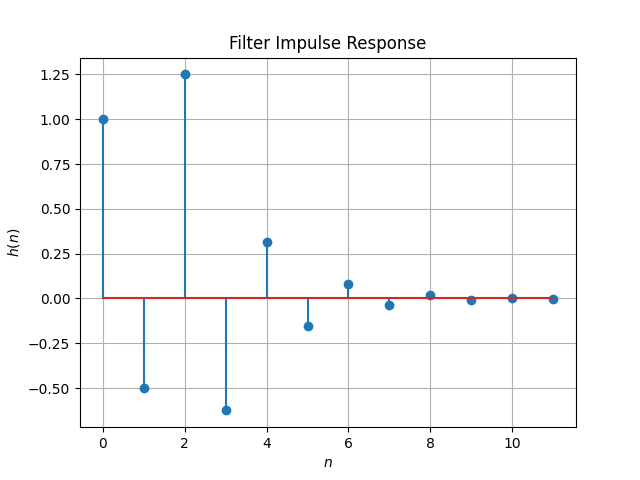
\includegraphics[width = \columnwidth]{figs/hn.png}
                \caption{$h\brak{n}$ as inverse of $H\brak{n}$}
                \label{hn}
           \end{figure}
           From the plot it seems like $h(n)$ is bounded and becomes smaller in magnitude as $n$ increases.\\
           Using $\eqref{eq:hn}$, we can get theoritical expression as,
           \begin{align}
                h\brak{n} & = \begin{cases}
                                   0                      & , n < 0     \\
                                   \brak{\frac{-1}{2}}^n  & , 0\leq n<2 \\
                                   5\brak{\frac{-1}{2}}^n & , n \geq 2
                              \end{cases}\label{eq:hn_theo}
           \end{align}
           A sequence $\cbrak{x_n}$ is said to be bounded if and only if there exist a positive real number $M$ such that,
           \begin{align}
                \abs{x_n} \leq M , \forall n \in \mathcal{N}\label{def:bounded}
           \end{align}
           So to say $h\brak{n}$ is bounded we should able to find the $M$ which satisfies $\eqref{def:bounded}$.\\
           For n < 0,
           \begin{align}
                \abs{h\brak{n}} \leq 0
           \end{align}
           For $0 \leq n <2$,
           \begin{align}
                \abs{h\brak{n}} & = \abs{\frac{-1}{2}}^{n}        \\
                                & = \brak{\frac{1}{2}}^{n} \leq 1
           \end{align}
           And for $n \geq 2$,
           \begin{align}
                \abs{h\brak{n}} & = \abs{5\brak{\frac{-1}{2}}}^{n}          \\
                                & = \brak{\frac{5}{2}}^{n} \leq \frac{5}{4}
           \end{align}
           From above three cases, we can get $M$ as,
           \begin{align}
                M & = max\cbrak{0,1,\frac{5}{4}} \\
                  & = \frac{5}{4}
           \end{align}
           Therefore, $h\brak{n}$ is bounded using $\eqref{def:bounded}$ with $M = \frac{5}{4}$ i.e.,
           \begin{align}
                \abs{h(n)} \leq \frac{5}{4}  \forall n \in \mathcal{N}
           \end{align}
     \item Convergent? Justify using the ratio test.\\
           \solution We can say a given real sequence $\cbrak{x_n}$ is convergent if
           \begin{align}
                \lim_{n \rightarrow \infty}\abs{\frac{x_{n+1}}{x_n}} < 1
           \end{align}
           This is known as Ratio test.\\
           In this case the limit will become,
           \begin{align}
                \lim_{n \rightarrow \infty}\abs{\frac{h\brak{n+1}}{h\brak{n}}} & = \lim_{n \rightarrow \infty}\abs{\frac{5\brak{\frac{-1}{2}}^{n+1}}{5\brak{\frac{-1}{2}}^{n}}} \\
                                                                               & = \lim_{n \rightarrow \infty}\abs{\frac{-1}{2}}                                                \\
                                                                               & = \frac{1}{2}
           \end{align}
           As $\frac{1}{2} < 1$, from root test we can say that $h\brak{n}$ is convergent.
     \item The system with $h(n)$ is defined to be stable if
           \begin{equation}
                \sum_{n=-\infty}^{\infty}h(n) < \infty
           \end{equation}
           Is the system defined by $\eqref{eq:iir_filter}$ stable for the impulse response in $\eqref{eq:impulse_resp}$?\\
           \solution From $\eqref{eq:hn}$,
           \begin{align}
                \sum_{n=-\infty}^{\infty}h\brak{n} & = \sum_{n=-\infty}^{\infty}\brak{\brak{\frac{-1}{2}}^{n} u\brak{n} + \brak{\frac{-1}{2}}^{n-2} u\brak{n-2}} \\
                                                   & = 2\brak{\frac{1}{1+\frac{1}{2}}}                                                                           \\
                                                   & = \frac{4}{3}
           \end{align}
           $\therefore$ the system is stable.
     \item Verify the above result using a python code.\\
           \solution Download the python code from the below link
           \begin{lstlisting}
wget https://github.com/Shivanshu8211/EE3900/blob/master/codes/hn_stable.py
\end{lstlisting}
           Then run the following command,
           \begin{lstlisting}
python3 hn_stable.py
\end{lstlisting}
     \item Compute and sketch $h(n)$ using
           \begin{equation}
                \label{eq:iir_filter_h}
                h(n) + \frac{1}{2}h(n-1) = \delta(n) + \delta(n-2),
           \end{equation}
           This is the definition of $h(n)$.\\
           \solution Download the code for the plot \ref{hndef} from the below link,
           \begin{lstlisting}
wget https://github.com/Shivanshu8211/EE3900/blob/master/codes/hndef.py
\end{lstlisting}
           Note that this is same as $\ref{hn}$.\\
           \begin{figure}[ht!]
                \centering
                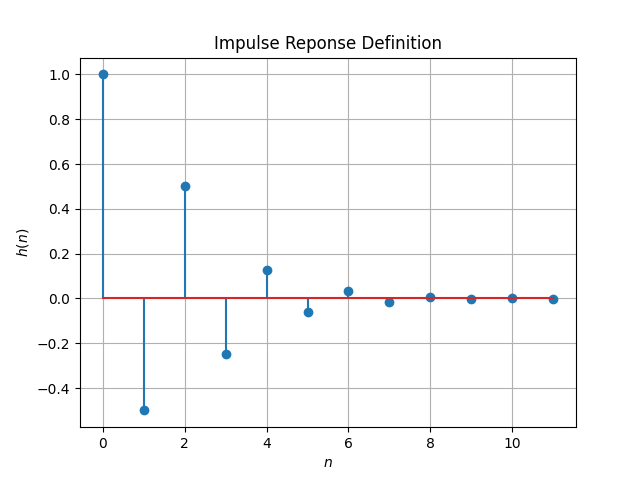
\includegraphics[width = \columnwidth]{figs/hndef.png}
                \caption{From the definition of $h(n)$}
                \label{hndef}
           \end{figure}
           For $n <0$, $h\brak{n} = 0$ and,
           \begin{align}
                h\brak{0} & = \delta\brak{0} \\
                          & = 1
           \end{align}
           For $n =1$,
           \begin{align}
                h\brak{1} + \frac{1}{2}h\brak{0} & = \delta\brak{1} + \delta\brak{-1} \\
                \implies  h\brak{1}              & = -\frac{1}{2}h\brak{0}            \\
                                                 & = -\frac{1}{2}
           \end{align}
           $n=2$,
           \begin{align}
                h\brak{2} + \frac{1}{2}h\brak{1} & = 0 + \delta\brak{0} \\
                h\brak{2}                        & = 1 + \frac{1}{4}    \\
                                                 & = \frac{5}{4}
           \end{align}
           And for $n>2$ RHS will be $0$ so,
           \begin{align}
                h\brak{n} & = -\frac{1}{2}h\brak{n-1}
           \end{align}
           Overall
           \begin{align}
                h\brak{n} & = \begin{cases}
                                   0                       & , n <0  \\
                                   1                       & , n = 0 \\
                                   -\frac{1}{2}            & , n=1   \\
                                   \frac{5}{4}             & , n =2  \\
                                   -\frac{1}{2}h\brak{n-1} & , n >2
                              \end{cases}
           \end{align}
     \item Compute
           %
           \begin{equation}
                \label{eq:convolution}
                y(n) = x(n)*h(n) = \sum_{k=-\infty}^{\infty}x(k)h(n-k)
           \end{equation}
           %
           Comment. The operation in $\eqref{eq:convolution}$ is known as
                {\em convolution}.\\
           %
           \solution Download the code for plot $\ref{ynconv}$ from the below link
           \begin{lstlisting}
wget https://github.com/Shivanshu8211/EE3900/blob/master/codes/ynconv.py
            \end{lstlisting}
           Note that the plot is same that as in $\ref{fig:xnyn}$.
           \begin{figure}[ht!]
                \centering
                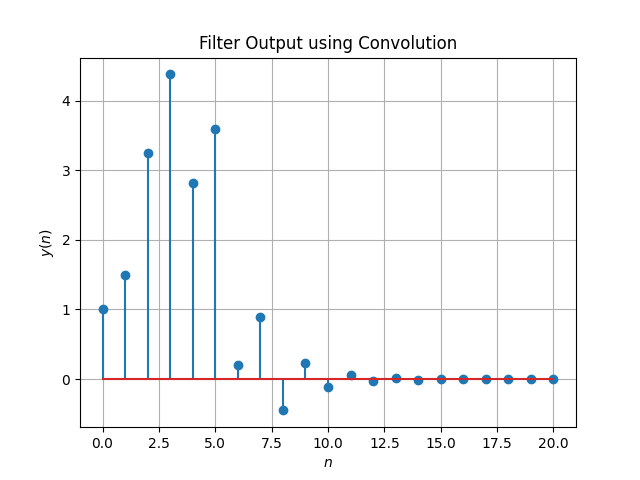
\includegraphics[width = \columnwidth]{figs/ynconv.png}
                \caption{$y(n)$ using the convolution definition}
                \label{ynconv}
           \end{figure}
     \item Express the above convolution using a Teoplitz matrix.\\
           \solution
           For finding the above convolution using topleitz matrix we have to find topleitz matrix of h(n).
           h(n) is tending to 0 for large n.
           So,we take upto some n only.
           So,
           \begin{align}
                h(n)=\myvec{1 \\-.5\\.\\.} \quad for \quad n=0,2 ...9
           \end{align}
           So,topleitz matrix of $h(n)$ will be
           \begin{align}
                top\{h(n)\}=\myvec{1 & 0 & 0 & 0 & 0 & 0 \\-.5 &1 &0 &0 &0 &0\\1.25&-.5&1&0&0&0\\. &.& .& .& .&. }
           \end{align}
           and
           \begin{align}
                x(n)=\myvec{1 \\2\\3\\4\\2\\1}
           \end{align}
           So,
           \begin{align}
                x(n)*h(n) & =top\{h(n)\}x(n) \\
                          & =\myvec{1        \\1.5\\3.25\\.\\.}
           \end{align}
     \item Show that\\
           \begin{equation}
                y(n) =  \sum_{k=-\infty}^{\infty}x(n-k)h(k)
           \end{equation}
           \solution Substitute $k := n-k$ in $\eqref{eq:convolution}$, we will get
           \begin{align}
                y(n) & = \sum_{k=-\infty}^{\infty}x(k)h(n-k)     \\
                     & = \sum_{n - k=-\infty}^{\infty}x(n-k)h(k) \\
                     & = \sum_{k = -\infty}^{\infty}x(n-k)h(k)
           \end{align}

\end{enumerate}
\section{DFT and FFT}
\begin{enumerate}[label=\thesection.\arabic*]
     \item
           Compute
           \begin{equation}
                X(k) \define \sum _{n=0}^{N-1}x(n) e^{-\j2\pi kn/N}, \quad k = 0,1,\dots, N-1
           \end{equation}
           and $H(k)$ using $h(n)$.\\
           \solution Download the below python code for the plot $\ref{DFT}$,
           \begin{lstlisting}
wget  https://github.com/Charanyash/EE3900-Digital_Signal_Processing/blob/master/Sound%201/Codes/dft.py
\end{lstlisting}
           And run the following command in the terminal,
           \begin{lstlisting}
python3 dft.py
\end{lstlisting}
           \begin{figure}[!h]
                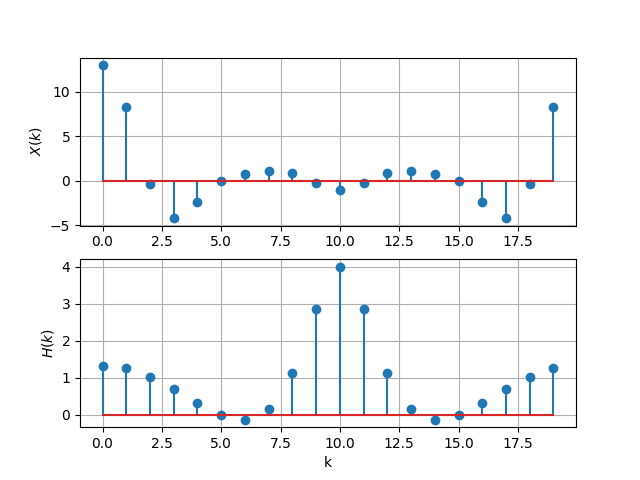
\includegraphics[width = \columnwidth]{figs/dft.png}
                \centering
                \caption{Plot of real part of Discrete Fourier Transforms of $x(n)$ and $h(n)$}
                \label{DFT}
           \end{figure}
     \item Compute
           \begin{equation}
                Y(k) = X(k)H(k)
           \end{equation}
           \solution Download the below python code for the plot $\ref{Y_k}$,
           \begin{lstlisting}
wget  https://github.com/Charanyash/EE3900-Digital_Signal_Processing/blob/master/Sound%201/Codes/Y_K.py
  \end{lstlisting}
           Then run the following command in the terminal,
           \begin{lstlisting}
python3 Y_K.py
 \end{lstlisting}
           \begin{figure}[!h]
                \centering
                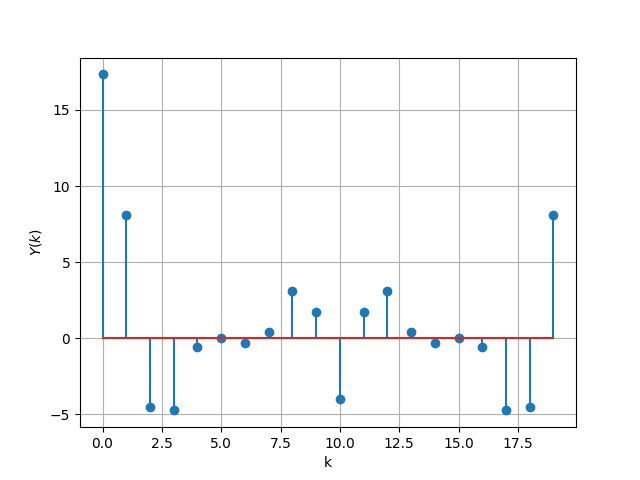
\includegraphics[width=\columnwidth]{figs/Y_k.png}
                \caption{$Y(k)$ as the product of $X(k)$ and $H(k)$}
                \label{Y_k}
           \end{figure}
     \item Compute
           \begin{equation}
                y\brak{n}={\frac {1}{N}}\sum _{k=0}^{N-1}Y\brak{k}\cdot e^{\j 2\pi kn/N},\quad n = 0,1,\dots, N-1
           \end{equation}
           \solution Download the below python code for the plot $\ref{yndft_dif}$,
           \begin{lstlisting}
wget https://github.com/Charanyash/EE3900-Digital_Signal_Processing/blob/master/Sound%201/Codes/yndft_dif.py
\end{lstlisting}
           Then run the following command,
           \begin{lstlisting}
python3 yndft_dif.py
 \end{lstlisting}
           \begin{figure}[!h]
                \centering
                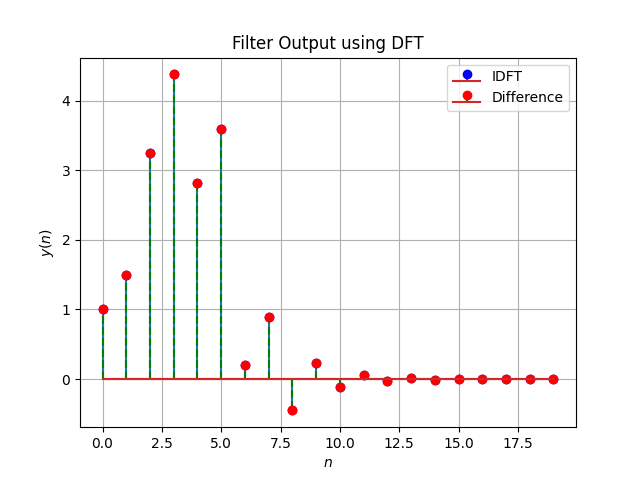
\includegraphics[width=\columnwidth]{figs/yndft_dif.png}
                \caption{$y(n)$ using IDFT and difference equation}
                \label{yndft_dif}
           \end{figure}
     \item Repeat the previous exercise by computing $X(k), H(k)$ and $y(n)$ through FFT and
           IFFT.\\
           \solution Download the below python code for the plot $\ref{yn_ifft}$,
           \begin{lstlisting}
wget https://github.com/Charanyash/EE3900-Digital_Signal_Processing/blob/master/Sound%201/Codes/yn_ifft.py
  \end{lstlisting}
           Then run the following command
           \begin{lstlisting}
python3 yn_ifft.py
   \end{lstlisting}
           \begin{figure}[!ht]
                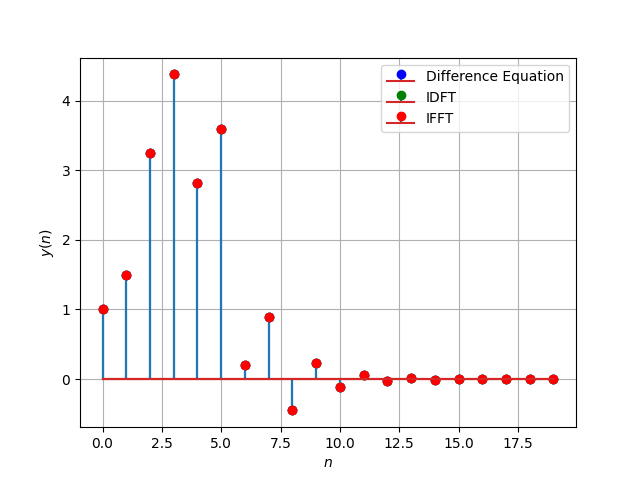
\includegraphics[width=\columnwidth]{figs/yn_ifft.png}
                \centering
                \caption{The plot of $y\brak{n}$ using IFFT}
                \label{yn_ifft}
           \end{figure}
\end{enumerate}
\section{FFT}
% \subsection{Definitions}
\begin{enumerate}[label=\arabic*.,ref=\thesection.\theenumi]
     \numberwithin{equation}{section}
     \item The DFT of $x(n)$ is given by
           \begin{align}
                X(k) \triangleq \sum_{n=0}^{N-1} x(n) e^{-j 2 \pi k n / N}, \quad k=0,1, \ldots, N-1
           \end{align}
     \item Let
           \begin{align}
                W_{N} = e^{-j2\pi/N}
           \end{align}
           Then the $N$-point {\em DFT matrix} is defined as
           \begin{align}
                \vec{F}_{N} = \sbrak{W_{N}^{mn}}, \quad 0 \le m,n \le N-1
           \end{align}
           where $W_{N}^{mn}$ are the elements of $\vec{F}_{N}$.
     \item Let
           \begin{align}
                \vec{I}_4 = \myvec{\vec{e}_4^{1} & \vec{e}_4^{2} & \vec{e}_4^{3} & \vec{e}_4^{4} }
           \end{align}
           be the $4\times 4$ identity matrix.  Then the 4 point {\em DFT permutation matrix} is defined as
           \begin{align}
                \vec{P}_4 = \myvec{\vec{e}_4^{1} & \vec{e}_4^{3} & \vec{e}_4^{2} & \vec{e}_4^{4} }
           \end{align}
     \item The 4 point {\em DFT diagonal matrix} is defined as
           \begin{align}
                \vec{D}_4 = diag\myvec{W_{4}^{0} & W_{N}^{1} & W_{N}^{2} & W_{N}^{3}}
           \end{align}
     \item Show that
           \begin{equation}
                W_{N}^{2}=W_{N/2} \label{fft-3}
           \end{equation}
           \solution Given that
           \begin{align}
                W_{N}     & = e^{-j2\pi/N}           \\
                W_{N}^{2} & = (e^{-j2\pi/N})^2       \\
                          & = e^{-j2\pi2/N}          \\
                          & = e^{-j2\pi/\frac{N}{2}} \\
                          & = W_{N/2}
           \end{align}
     \item Show that
           \begin{equation}
                \vec{F}_{4}=
                \begin{bmatrix}
                     \vec{I}_{2} & \vec{D}_{2}  \\
                     \vec{I}_{2} & -\vec{D}_{2}
                \end{bmatrix}
                \begin{bmatrix}
                     \vec{F}_{2} & 0           \\
                     0           & \vec{F}_{2}
                \end{bmatrix}
                \vec{P}_{4}
           \end{equation}
           \solution Taking R.H.S.
           \begin{equation}
                R.H.S. =
                \begin{bmatrix}
                     \vec{I}_{2} & \vec{D}_{2}  \\
                     \vec{I}_{2} & -\vec{D}_{2}
                \end{bmatrix}
                \begin{bmatrix}
                     \vec{F}_{2} & 0           \\
                     0           & \vec{F}_{2}
                \end{bmatrix} \\
                \vec{P}_{4}
           \end{equation}
           \begin{equation}
                =
                \begin{bmatrix}
                     \vec{F}_{2} & \vec{D}_{2}\vec{F}_{2}  \\
                     \vec{F}_{2} & -\vec{D}_{2}\vec{F}_{2}
                \end{bmatrix}
                \vec{P}_{4}
           \end{equation}
           \begin{equation}
                =
                \begin{bmatrix}
                     1 & 1  & 1  & 1  \\
                     1 & -1 & -i & i  \\
                     1 & 1  & -1 & -1 \\
                     1 & -1 & i  & -i
                \end{bmatrix}
                \vec{P}_{4}
           \end{equation}
           \begin{equation}
                =
                \begin{bmatrix}
                     1 & 1  & 1  & 1  \\
                     1 & -1 & -i & i  \\
                     1 & 1  & -1 & -1 \\
                     1 & -1 & i  & -i
                \end{bmatrix}
                \begin{bmatrix}
                     1 & 0 & 0 & 0 \\
                     0 & 0 & 1 & 0 \\
                     0 & 1 & 0 & 0 \\
                     0 & 0 & 0 & 1 \\
                \end{bmatrix}
           \end{equation}
           \begin{equation}
                =
                \begin{bmatrix}
                     1 & 1  & 1  & 1  \\
                     1 & -i & -1 & i  \\
                     1 & -1 & 1  & -1 \\
                     1 & i  & -1 & -i
                \end{bmatrix}
           \end{equation}
           \begin{equation}
                = \vec{F}_{4}
           \end{equation}
     \item Show that
           \begin{equation}
                \vec{F}_{N}=
                \begin{bmatrix}
                     \vec{I}_{N/2} & \vec{D}_{N/2}  \\
                     \vec{I}_{N/2} & -\vec{D}_{N/2}
                \end{bmatrix}
                \begin{bmatrix}
                     \vec{F}_{N/2} & 0             \\
                     0             & \vec{F}_{N/2}
                \end{bmatrix}
                \vec{P}_{N}
           \end{equation}
           \solution
           For N even ;
           We already know ;
           \begin{align}
                \vec{F}_{N} = \sbrak{W_{N}^{mn}}, \quad 0 \le m,n \le N-1 \\
                \vec{D}_{N}\vec{F}_{N} = \sbrak{W_{N}^{m.(2k+1)}}, \quad 0 \le m,k \le \frac{N}{2}-1
           \end{align}
           \begin{align}
                \vec{F}_{N}\vec{P}_{N} & =\begin{bmatrix}
                                               {W_{N}^{2mk}} & {W_{N}^{m.(2k+1)}} \\ {W_{N}^{2mk+Nk}}&{W_{N}^{m.(2k+1)+\frac{N}{2}.(2k+1)}}
                                          \end{bmatrix}  \nonumber \\
                                       & \quad \quad \quad \quad \quad 0 \le m,k \le \frac{N}{2}-1  \nonumber                                                     \\
                \vec{F}_{N}\vec{P}_{N} & =\begin{bmatrix}
                                               {W_{N}^{2mk}} & {W_{N}^{m.(2k+1)}} \\ {W_{N}^{2mk}}&-{W_{N}^{m.(2k+1)}}
                                          \end{bmatrix}
           \end{align}
           from \eqref{fft-3} ;
           \begin{align}
                \vec{F}_{N}\vec{P}_{N} & =\begin{bmatrix}
                                               {W_{N/2}^{mk}} & {W_{N/2}^{m.(k+1/2)}} \\ {W_{N/2}^{mk}}&-{W_{N}^{m.(k+1/2)}}
                                          \end{bmatrix} \\
                \vec{F}_{N}\vec{P}_{N} & =\begin{bmatrix}
                                               \vec{F}_{N/2} & \vec{D}_{N/2}\vec{F}_{N/2} \\ \vec{F}_{N/2}&-\vec{D}_{N/2}\vec{F}_{N/2}
                                          \end{bmatrix}
           \end{align}
           Also we know that
           \begin{align}
                \vec{P}_{N}^2 = \vec{I}_{N} \label{fft-4}
           \end{align}
           \begin{align}
                \vec{F}_{N} & =\begin{bmatrix}
                                    \vec{F}_{N/2} & \vec{D}_{N/2}\vec{F}_{N/2} \\ \vec{F}_{N/2}&-\vec{D}_{N/2}\vec{F}_{N/2}
                               \end{bmatrix} \vec{P}_{N}
           \end{align}
           From above it follows ;
           \begin{equation}
                \vec{F}_{N}=
                \begin{bmatrix}
                     \vec{I}_{N/2} & \vec{D}_{N/2}  \\
                     \vec{I}_{N/2} & -\vec{D}_{N/2}
                \end{bmatrix}
                \begin{bmatrix}
                     \vec{F}_{N/2} & 0             \\
                     0             & \vec{F}_{N/2}
                \end{bmatrix}
                \vec{P}_{N}
           \end{equation}
     \item Find
           \begin{align}
                \vec{P}_4 \vec{x}
           \end{align}
           \solution We know that
           \begin{align}
                x(n)=\myvec{1 \\2\\3\\4\\2\\1}
           \end{align}
           So,
           \begin{equation}
                \vec{P}_4 \vec{x} =
                \begin{bmatrix}
                     1 & 0 & 0 & 0 & 0 & 0 \\
                     0 & 0 & 1 & 0 & 0 & 0 \\
                     0 & 1 & 0 & 0 & 0 & 0 \\
                     0 & 0 & 0 & 1 & 0 & 0 \\
                \end{bmatrix}
                \begin{bmatrix}
                     1 \\
                     2 \\
                     3 \\
                     4 \\
                     2 \\
                     1 \\
                \end{bmatrix}
           \end{equation}
           \begin{equation}
                =
                \begin{bmatrix}
                     1 & 3 & 2 & 4
                \end{bmatrix}
           \end{equation}
     \item Show that
           \begin{align}
                \vec{X} = \vec{F}_N \vec{x}
                \label{eq:dft-mat-def}
           \end{align}
           \solution
           We know that \\
           \begin{align}
                X(k) \triangleq \sum_{n=0}^{N-1} x(n) e^{-j 2 \pi k n / N}, \quad k=0,1, \ldots, N-1 \\
           \end{align}
           where $\vec{x}, \vec{X}$ are the vector representations of $x(n), X(k)$ respectively.
           \begin{equation}
                \vec{X} =
                \begin{bmatrix}
                     x(0)e^{-j 2 \pi k 0 / N} \\
                     x(1)e^{-j 2 \pi k 1 / N} \\
                     x(2)e^{-j 2 \pi k 2 / N} \\
                     .                        \\
                     .                        \\
                     .                        \\
                     x(n)e^{-j 2 \pi k n / N}
                \end{bmatrix}
           \end{equation}
           \begin{equation}
                \vec{P}_N \vec{x} =
                \begin{bmatrix}
                     W_N^{0\times0}     & W_N^{0\times1}     & .. & W_N^{0\times N-1}    \\
                     ..                 & ..                 & .. & ..                   \\
                     W_N^{N-1 \times 0} & W_N^{N-1 \times 1} & .. & W_N^{N-1 \times N-1}
                \end{bmatrix}
                \begin{bmatrix}
                     x(0)   \\
                     x(1)   \\
                     x(2)   \\
                     .      \\
                     .      \\
                     x(n-1) \\
                \end{bmatrix}
           \end{equation}
           \begin{equation}
                \begin{bmatrix}
                     \sum_{n=0}^{N-1}W_N^{0\times n} x(n) \\
                     \sum_{n=0}^{N-1}W_N^{1\times n} x(n) \\
                     .                                    \\
                     .                                    \\
                     \sum_{n=0}^{N-1}W_N^{N-1\times n} x(n)
                \end{bmatrix}
           \end{equation}
           \begin{equation}
                \begin{bmatrix}
                     \sum_{n=0}^{N-1}e^{\frac{-j2\pi0\times n}{N}} x(n) \\
                     \sum_{n=0}^{N-1}e^{\frac{-j2\pi1\times n}{N}} x(n) \\
                     .                                                  \\
                     .                                                  \\
                     \sum_{n=0}^{N-1}e^{\frac{-j2\pi (N-1)\times n}{N}} x(n)
                \end{bmatrix}
           \end{equation}
           \begin{align}
                 & =\vec{X}
           \end{align}
     \item Derive the following Step-by-step visualisation  of
           8-point FFTs into 4-point FFTs and so on
           \begin{equation}
                \begin{bmatrix}
                     X(0) \\
                     X(1) \\
                     X(2) \\
                     X(3)
                \end{bmatrix}
                =
                \begin{bmatrix}
                     X_{1}(0) \\
                     X_{1}(1) \\
                     X_{1}(2) \\
                     X_{1}(3) \\
                \end{bmatrix}
                +
                \begin{bmatrix}
                     W^{0}_{8} & 0         & 0         & 0         \\
                     0         & W^{1}_{8} & 0         & 0         \\
                     0         & 0         & W^{2}_{8} & 0         \\
                     0         & 0         & 0         & W^{3}_{8}
                \end{bmatrix}
                \begin{bmatrix}
                     X_{2}(0) \\
                     X_{2}(1) \\
                     X_{2}(2) \\
                     X_{2}(3)
                \end{bmatrix}
           \end{equation}
           \begin{equation}
                \begin{bmatrix}
                     X(4) \\
                     X(5) \\
                     X(6) \\
                     X(7)
                \end{bmatrix}
                =
                \begin{bmatrix}
                     X_{1}(0) \\
                     X_{1}(1) \\
                     X_{1}(2) \\
                     X_{1}(3) \\
                \end{bmatrix}
                -
                \begin{bmatrix}
                     W^{0}_{8} & 0         & 0         & 0         \\
                     0         & W^{1}_{8} & 0         & 0         \\
                     0         & 0         & W^{2}_{8} & 0         \\
                     0         & 0         & 0         & W^{3}_{8}
                \end{bmatrix}
                \begin{bmatrix}
                     X_{2}(0) \\
                     X_{2}(1) \\
                     X_{2}(2) \\
                     X_{2}(3)
                \end{bmatrix}
           \end{equation}
           4-point FFTs into 2-point FFTs
           \begin{equation}
                \begin{bmatrix}
                     X_{1}(0) \\
                     X_{1}(1) \\
                \end{bmatrix}
                =
                \begin{bmatrix}
                     X_{3}(0) \\
                     X_{3}(1) \\
                \end{bmatrix}
                +
                \begin{bmatrix}
                     W^{0}_{4} & 0         \\
                     0         & W^{1}_{4}
                \end{bmatrix}
                \begin{bmatrix}
                     X_{4}(0) \\
                     X_{4}(1) \\
                \end{bmatrix}
           \end{equation}
           \begin{equation}
                \begin{bmatrix}
                     X_{1}(2) \\
                     X_{1}(3) \\
                \end{bmatrix}
                =
                \begin{bmatrix}
                     X_{3}(0) \\
                     X_{3}(1) \\
                \end{bmatrix}
                -
                \begin{bmatrix}
                     W^{0}_{4} & 0         \\
                     0         & W^{1}_{4}
                \end{bmatrix}
                \begin{bmatrix}
                     X_{4}(0) \\
                     X_{4}(1) \\
                \end{bmatrix}
           \end{equation}
           \begin{equation}
                \begin{bmatrix}
                     X_{2}(0) \\
                     X_{2}(1) \\
                \end{bmatrix}
                =
                \begin{bmatrix}
                     X_{5}(0) \\
                     X_{5}(1) \\
                \end{bmatrix}
                +
                \begin{bmatrix}
                     W^{0}_{4} & 0         \\
                     0         & W^{1}_{4}
                \end{bmatrix}
                \begin{bmatrix}
                     X_{6}(0) \\
                     X_{6}(1) \\
                \end{bmatrix}
           \end{equation}
           \begin{equation}
                \begin{bmatrix}
                     X_{2}(2) \\
                     X_{2}(3) \\
                \end{bmatrix}
                =
                \begin{bmatrix}
                     X_{5}(0) \\
                     X_{5}(1) \\
                \end{bmatrix}
                -
                \begin{bmatrix}
                     W^{0}_{4} & 0         \\
                     0         & W^{1}_{4}
                \end{bmatrix}
                \begin{bmatrix}
                     X_{6}(0) \\
                     X_{6}(1) \\
                \end{bmatrix}
           \end{equation}
           \begin{equation}
                P_{8}
                \begin{bmatrix}
                     x(0) \\
                     x(1) \\
                     x(2) \\
                     x(3) \\
                     x(4) \\
                     x(5) \\
                     x(6) \\
                     x(7)
                \end{bmatrix}
                =
                \begin{bmatrix}
                     x(0) \\
                     x(2) \\
                     x(4) \\
                     x(6) \\
                     x(1) \\
                     x(3) \\
                     x(5) \\
                     x(7)
                \end{bmatrix}
           \end{equation}
           \begin{equation}
                P_{4}
                \begin{bmatrix}
                     x(0) \\
                     x(2) \\
                     x(4) \\
                     x(6) \\
                \end{bmatrix}
                =
                \begin{bmatrix}
                     x(0) \\
                     x(4) \\
                     x(2) \\
                     x(6)
                \end{bmatrix}
           \end{equation}
           \begin{equation}
                P_{4}
                \begin{bmatrix}
                     x(1) \\
                     x(3) \\
                     x(5) \\
                     x(7)
                \end{bmatrix}
                =
                \begin{bmatrix}
                     x(1) \\
                     x(5) \\
                     x(3) \\
                     x(7) \\
                \end{bmatrix}
           \end{equation}
           Therefore,
           \begin{equation}
                \begin{bmatrix}
                     X_{3}(0) \\
                     X_{3}(1) \\
                \end{bmatrix}
                = F_{2}
                \begin{bmatrix}
                     x(0) \\
                     x(4) \\
                \end{bmatrix}
           \end{equation}
           \begin{equation}
                \begin{bmatrix}
                     X_{4}(0) \\
                     X_{4}(1) \\
                \end{bmatrix}
                = F_{2}
                \begin{bmatrix}
                     x(2) \\
                     x(6) \\
                \end{bmatrix}
           \end{equation}
           \begin{equation}
                \begin{bmatrix}
                     X_{5}(0) \\
                     X_{5}(1) \\
                \end{bmatrix}
                = F_{2}
                \begin{bmatrix}
                     x(1) \\
                     x(5) \\
                \end{bmatrix}
           \end{equation}
           \begin{equation}
                \begin{bmatrix}
                     X_{6}(0) \\
                     X_{6}(1) \\
                \end{bmatrix}
                = F_{2}
                \begin{bmatrix}
                     x(3) \\
                     x(7) \\
                \end{bmatrix}
           \end{equation}
     \item For
           \begin{align}
                \vec{x} = \myvec{1 \\2\\3\\4\\2\\1}
                \label{eq:equation1}
           \end{align}
           compte the DFT
           using \\
           \eqref{eq:dft-mat-def}
           \solution Let N=6. So,
           \begin{align}
                 & \vec{X}=\vec{F}_6\vec{x}                                                                                                                          \\
                 & =\begin{bmatrix}
                         W_6^{mn}
                    \end{bmatrix}\vec{x}                                                                                                                             \\
                 & =\begin{bmatrix}
                         W_6^0 & W_6^0 & W_6^0    & W_6^0    & W_6^0    & W_6^0    \\
                         W_6^0 & W_6^1 & W_6^2    & W_6^3    & W_6^4    & W_6^5    \\
                         W_6^0 & W_6^2 & W_6^4    & W_6^6    & W_6^8    & W_6^{10} \\
                         W_6^0 & W_6^3 & W_6^6    & W_6^9    & W_6^{12} & W_6^{15} \\
                         W_6^0 & W_6^4 & W_6^8    & W_6^{12} & W_6^{16} & W_6^{20} \\
                         W_6^0 & W_6^5 & W_6^{10} & W_6^{15} & W_6^{20} & W_6^{25} \\
                    \end{bmatrix}\vec{x}                                                                                        \\
                 & =\begin{bmatrix}
                         1 & 1                    & 1                     & 1          & 1                     & 1                   \\
                         1 & e^{-j\frac{\pi}{3}}  & e^{-j\frac{2\pi}{3}}  & e^{-j\pi}  & e^{-j\frac{4\pi}{3}}  & e^{\frac{5\pi}{3}}  \\
                         1 & e^{-j\frac{2\pi}{3}} & e^{-j\frac{4\pi}{3}}  & e^{-j2\pi} & e^{-j\frac{8\pi}{3}}  & e^{\frac{10\pi}{3}} \\
                         1 & e^{-j\pi}            & e^{-j2\pi}            & e^{-j3\pi} & e^{-j4\pi}            & e^{-j5\pi}          \\
                         1 & e^{-j\frac{4\pi}{3}} & e^{-j\frac{8\pi}{3}}  & e^{-j4\pi} & e^{-j\frac{16\pi}{3}} & e^{\frac{20\pi}{3}} \\
                         1 & e^{-j\frac{5\pi}{3}} & e^{-j\frac{10\pi}{3}} & e^{-j5\pi} & e^{-j\frac{20\pi}{3}} & e^{\frac{25\pi}{3}} \\
                    \end{bmatrix}\myvec{1 \\2\\3\\4\\2\\1}\\
                 & =\myvec{13+0j                                                                                                                                     \\
                -4-1.732j                                                                                                                                            \\
                1+0j                                                                                                                                                 \\
                -1+0j                                                                                                                                                \\
                1+0j                                                                                                                                                 \\
                     -4+1.732j}
           \end{align}
           Download and run the following python program.
           \begin{lstlisting}
wget https://github.com/Shivanshu8211/EE3900/blob/master/codes/dft_fx.py
           \end{lstlisting}
     \item Repeat the above exercise using the FFT
           after zero padding $\vec{x}$. \\
           \solution  We know that FFT works for N  which is of the form $2^n$ where $n\in \cal N$.
           So, we have to pad $\vec{x}$ with zeros to its nearest $2^n$ length.
           So,
           \begin{align}
                \vec{x}=\myvec{1 \\2\\3\\4\\2\\1\\0\\0}
           \end{align}
           We know that if N is even then
           \begin{align}
                \vec{F}_N & =\begin{bmatrix}
                                  \vec{F}_{N/2} & \vec{D}_{N/2}\vec{F}_{N/2}  \\
                                  \vec{F}_{N/2} & -\vec{D}_{N/2}\vec{F}_{N/2}
                             \end{bmatrix}\vec{P}_N
           \end{align}
           So,
           \begin{align}
                \vec{F}_2 & =\begin{bmatrix}
                                  \vec{F}_{1} & \vec{D}_{1}\vec{F}_{1}  \\
                                  \vec{F}_{1} & -\vec{D}_{1}\vec{F}_{1}
                             \end{bmatrix}\vec{P}_2 \\
                          & =\begin{bmatrix}
                                  1 & 1  \\
                                  1 & -1
                             \end{bmatrix}
                \begin{bmatrix}
                     1 & 0 \\
                     0 & 1
                \end{bmatrix}                                     \\
                          & =\begin{bmatrix}
                                  1 & 1  \\
                                  1 & -1
                             \end{bmatrix}
           \end{align}
           Now,
           \begin{align}
                \vec{D}_{2}\vec{F}_{2} & =diag\myvec{W_{4}^{0} & W_{4}^{1}}\vec{F}_{2} \\
                                       & =\begin{bmatrix}
                                               1 & 0  \\
                                               0 & -j
                                          \end{bmatrix}
                \begin{bmatrix}
                     1 & 1  \\
                     1 & -1
                \end{bmatrix}                                                         \\
                                       & =\begin{bmatrix}
                                               1  & 1 \\
                                               -j & j
                                          \end{bmatrix}
           \end{align}
           So,
           \begin{align}
                \vec{F}_4 & =\begin{bmatrix}
                                  \vec{F}_{2} & \vec{D}_{2}\vec{F}_{2}  \\
                                  \vec{F}_{2} & -\vec{D}_{2}\vec{F}_{2}
                             \end{bmatrix}\vec{P}_4 \\
                          & =\begin{bmatrix}
                                  1 & 1  & 1  & 1  \\
                                  1 & -1 & -j & j  \\
                                  1 & 1  & -1 & -1 \\
                                  1 & -1 & j  & -j
                             \end{bmatrix}\begin{bmatrix}
                                               1 & 0 & 0 & 0 \\
                                               0 & 0 & 1 & 0 \\
                                               0 & 1 & 0 & 0 \\
                                               0 & 0 & 0 & 1 \\
                                          \end{bmatrix}           \\
                          & =\begin{bmatrix}
                                  1 & 1  & 1  & 1  \\
                                  1 & -j & -1 & j  \\
                                  1 & -1 & 1  & -1 \\
                                  1 & j  & -1 & -j \\
                             \end{bmatrix}
           \end{align}
           Now,
           \begin{align}
                \vec{D}_{4}\vec{F}_{4} & =diag\myvec{W_{8}^{0} & W_{8}^{1} & W_{8}^{2} & W_{8}^{3}}\vec{F}_{4} \\
                                       & =
           \end{align}
           %	    \eqref{eq:fft-mat-def}
     \item Write a C program to compute the 8-point FFT. \\
           \solution Download and run the following C program.
           \begin{lstlisting}
wget https://github.com/Shivanshu8211/EE3900/blob/master/codes/8point_fft.c
           \end{lstlisting}
     \end{enumerate}
     
     \section{Exercises}
     Answer the following questions by looking at the python code in Problem \ref{prob:output}
     \begin{enumerate}[label=\thesection.\arabic*]
          \item The command
               \begin{lstlisting}
output_signal = signal.lfilter(b, a, input_signal)
               \end{lstlisting}
               in Problem \ref{prob:output} is executed through the following difference equation
               \begin{equation}
                    \label{eq:iir_filter_gen}
                    \sum _{m=0}^{M}a\brak{m}y\brak{n-m}=\sum _{k=0}^{N}b\brak{k}x\brak{n-k}
               \end{equation}
               where the input signal is $x(n)$ and the output signal is $y(n)$ with initial values all 0. Replace \textbf{signal.filtfilt} with your own routine and verify.

               \solution On taking the $Z$-transform on both sides of the difference equation
               \begin{align}
                    \sum _{m=0}^{M}a\brak{m} z^{-m} Y(z) & = \sum _{k=0}^{N}b\brak{k} z^{-k} X(z)                                    \\
                    \implies H(z) = \frac{Y(z)}{X(z)}    & = \frac{\sum _{k=0}^{N}b\brak{k} z^{-k}}{\sum _{m=0}^{M}a\brak{m} z^{-m}}
               \end{align}

               For obtaining the discrete Fourier transform, put $z = \j \frac{2\pi i}{I}$ where $I$ is the length of the input signal and $i = 0, 1, \ldots, I-1$

               Download the following Python code that does the above
               \begin{lstlisting}
wget https://github.com/karthik6281/Signal-Processing/tree/main/Assignment1/codes/8_1.c
               \end{lstlisting}

               Run the code by executing
               \begin{lstlisting}
python3 8_1.py
               \end{lstlisting}

          \item Repeat all the exercises in the previous sections for the above $a$ and $b$

               \solution The polynomial coefficients obtained are
               \begin{align}
                    \vec{a} = \myvec{1.000 \\ -2.519 \\ 2.561 \\ -1.206 \\ 0.220} \qquad
                    \vec{b} = \myvec{0.003 \\ 0.014 \\ 0.021 \\ 0.014 \\ 0.003}
               \end{align}

               The difference equation is then given by
               \begin{equation}
                    \vec{a}^\top \vec{y} = \vec{b}^\top \vec{x}
               \end{equation}

               where
               \begin{align}
                    \vec{y} = \myvec{y(n) \\ y(n-1) \\ y(n-2) \\ y(n-3) \\ y(n-4)} \qquad
                    \vec{x} = \myvec{x(n) \\ x(n-1) \\ x(n-2) \\ x(n-3) \\ x(n-4)}
               \end{align}

               We have
               \begin{equation}
                    H(z) = \frac{Y(z)}{X(z)} = \frac{\sum _{k=0}^{N}b\brak{k} z^{-k}}{\sum _{m=0}^{M}a\brak{m} z^{-m}}
               \end{equation}

               By using partial fraction decomposition, we can write this as
               \begin{equation}
                    H(z) = \sum_i \frac{r(i)}{1-p(i)z^{-1}} + \sum_j k(j)z^{-j}
               \end{equation}

               On taking the inverse $Z$-transform on both sides by using \eqref{eq:anun}
               \begin{align}
                    H(z)                   & \ztrans h(n)              \\
                    \frac{1}{1-p(i)z^{-1}} & \ztrans \brak{p(i)}^nu(n) \\
                    z^{-j}                 & \ztrans \delta(n-j)
               \end{align}

               Thus
               \begin{align}
                    h(n) = \sum_i r(i)\brak{p(i)}^nu(n) + \sum_j k(j)\delta(n-j)
               \end{align}

               Download the following Python code
               \begin{lstlisting}
wget https://github.com/karthik6281/Signal-Processing/tree/main/Assignment1/codes/8_2.py
                    \end{lstlisting}

               Run the code by executing
               \begin{lstlisting}
python3 8_2.py
               \end{lstlisting}

               The above code outputs the values of $r(i), p(i), k(i)$
               \begin{multline}
                    h(n) =
                    \Re\brak{(0.24 - 0.71\j)(0.56 + 0.14\j)^n} u(n) \\
                    + \Re\brak{(0.24 + 0.71\j)(0.56 - 0.14\j)^n} u(n) \\
                    + 0.016\delta(n)
               \end{multline}

               \begin{figure}[!ht]
                    \centering
                    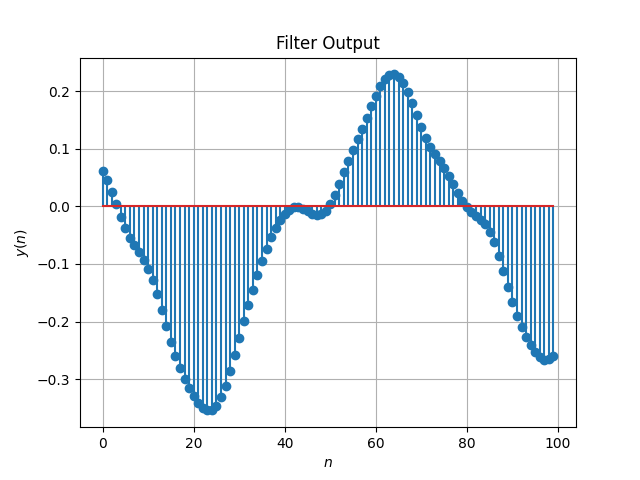
\includegraphics[width=\columnwidth]{./figs/8_2_1.png}
                    \caption{Plot of $y(n)$}
                    \label{fig-8.2.1}
               \end{figure}

               \begin{figure}[!ht]
                    \centering
                    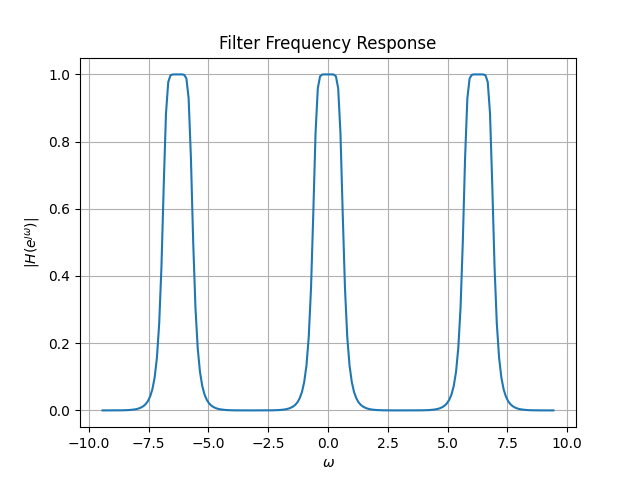
\includegraphics[width=\columnwidth]{./figs/8_2_2.png}
                    \caption{Plot of $\abs{H(e^{j\omega})}$}
                    \label{fig-8.2.2}
               \end{figure}

               \begin{figure}[!ht]
                    \centering
                    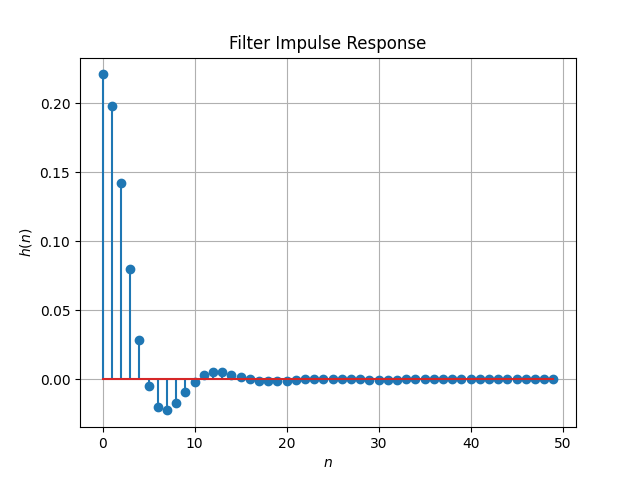
\includegraphics[width=\columnwidth]{./figs/8_2_3.png}
                    \caption{Plot of $h(n)$}
                    \label{fig-8.2.3}
               \end{figure}

          \item
               What is type, order and  cutoff-frequency of the above butterworth filter

               \solution
               The given butterworth filter is low pass with order=4 and cutoff-frequency=4kHz.
               %
          \item
               Modifying the code with different input parameters and to get the best possible output.
               %
               \solution
               Order: 10
               Cutoff frequency: 3000 Hz
     \end{enumerate}
\end{document}

